\chapter{Fundamentação Teórica}
Este capitulo busca contextualizar os principais conceitos abordados no presente trabalho, tais como os materiais utilizados como base e também a tecnologia adotada no desenvolvimento do projeto. E ao final, serão elencados alguns trabalhos correlatos.

\section{ENEF}
A Estratégia Nacional de Educação Financeira (ENEF) representa uma resposta proativa e estruturada às crescentes demandas de uma sociedade que enfrenta desafios financeiros complexos. Instituída com o claro objetivo de aprimorar a conscientização financeira da população brasileira, a ENEF busca não apenas promover a cidadania, mas também equipar os indivíduos com as ferramentas necessárias para tomar decisões financeiras informadas.

Esta estratégia abrange um amplo espectro de áreas de estudo, que vão desde os direitos e deveres básicos até tópicos mais complexos, como investimentos, previdência e planejamento financeiro. A inclusão de temas como poupança, crédito, seguros e consumo demonstra a abordagem abrangente adotada pela ENEF. Ao abordar temas tão variados, a ENEF reconhece e enfatiza que a educação financeira é um processo contínuo, que deve começar na infância e continuar ao longo da vida.

\subsection{Material Didático}
A ENEF destaca-se por sua abordagem prática, evidenciada por sua ampla variedade de materiais didáticos. Foram elaborados 24 livros especificamente alinhados com a missão educacional da ENEF. Cada livro foi cuidadosamente desenvolvido para atender às necessidades de diferentes faixas etárias: 18 destinados ao Ensino Fundamental e os 6 restantes focados no Ensino Médio. Uma característica notável é a separação dos livros em materiais específicos para alunos e guias para professores, garantindo que o conteúdo seja adequadamente direcionado para cada público.

Os primeiros livros têm como objetivo familiarizar os alunos do Ensino Fundamental com conceitos fundamentais de cidadania. Através de situações cotidianas, como a organização de uma sala de aula ou a coordenação de eventos escolares, os alunos são introduzidos a princípios de planejamento e organização. Conforme avançam na série, são gradualmente expostos a temas financeiros mais sofisticados, desde o entendimento básico das contas domésticas até a compreensão da origem e da trajetória do dinheiro na sociedade.

Dentre os materiais didáticos, os livros-jogo se destacam por suas narrativas envolventes. Ao invés de simplesmente transmitir informações, esses livros contam histórias que permitem aos alunos explorar cenários financeiros e entender as consequências de várias decisões. Esse enfoque narrativo é enriquecido por discussões em livros subsequentes, que oferecem insights sobre o papel de diferentes instituições financeiras e seu impacto na sociedade.

Nos 5º e 6º livros da série ENEF, observa-se uma abordagem pedagógica inovadora e envolvente, que reflete a excelência e o comprometimento da ENEF em proporcionar uma educação financeira de qualidade. Estes volumes adotam um formato interativo chamado "livro-jogo". Enquanto o jogo digital foca na jogabilidade, o livro-jogo se destaca por sua capacidade de envolver o leitor em uma narrativa rica, permitindo-lhe tomar decisões que influenciam os rumos da história.

A Figura 1 ilustra um esquema que destaca alguns dos caminhos possíveis que a história pode seguir. Este diagrama demonstra a complexidade e a diversidade de trajetórias que um jogador pode experimentar, refletindo diferentes escolhas financeiras e suas respectivas consequências.

As Figuras 2 e 3 retratam momentos cruciais na narrativa do livro-jogo. Em cada figura, o leitor é introduzido a um cenário e, posteriormente, confrontado com duas ou três opções de ação. Cada escolha desencadeia diferentes desenvolvimentos na história, ilustrando as implicações de suas decisões no mundo financeiro.

Na continuação da série, principalmente nas fases finais do Ensino Fundamental, a ENEF aprofunda a abordagem, introduzindo conceitos mais avançados e específicos sobre o universo financeiro. Os alunos são expostos a uma variedade de instituições financeiras e suas respectivas funções. Por exemplo, ao aprender sobre bancos, os estudantes ganham insights sobre operações bancárias, sistemas de crédito e a importância da gestão financeira. Quando o tema é agências de viagens ou hotéis, os alunos são introduzidos ao mundo das transações comerciais, tarifas, reservas e a economia do turismo. Essa abordagem detalhada serve para ampliar o horizonte dos alunos e prepará-los para interações financeiras mais complexas no futuro.

\begin{figure}[h]
	\centering
	\caption{Esquema com alguns dos caminhos possíveis da primeiro jogo/história.}
	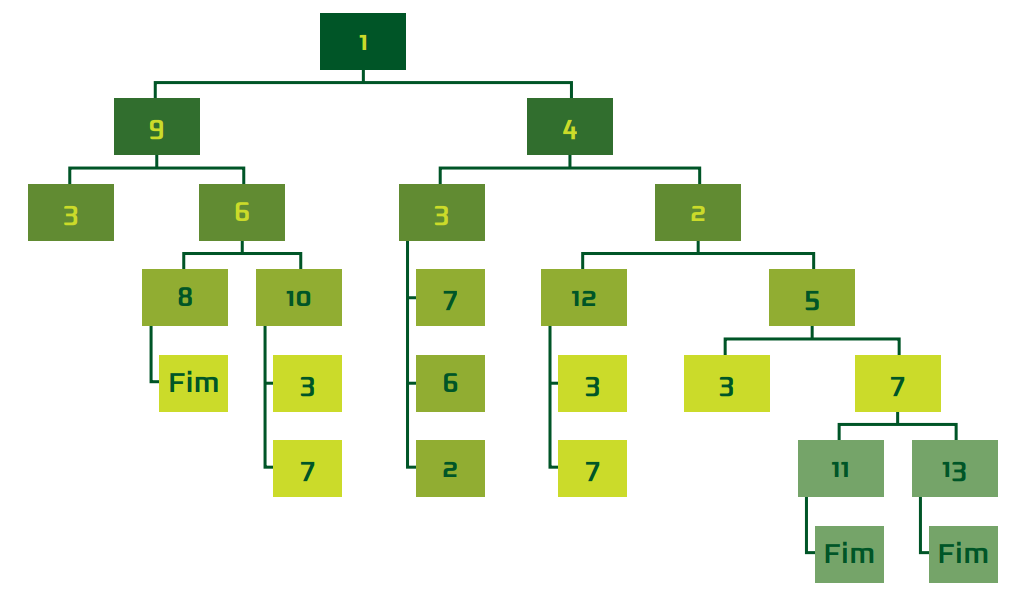
\includegraphics[scale=0.3]{Textuais/Pictures/Picture1.png}
	\fonte{\cite{Educacao_financeira_nas_escolas_professor}}\label{fig:figure-1}
\end{figure}
\begin{figure}[h]
	\centering
	\caption{Momento de decisão com duas possibilidades de caminhos.}
	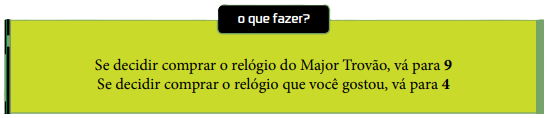
\includegraphics[scale=1]{Textuais/Pictures/Picture2.png}
	\fonte{\cite{Educacao_financeira_nas_escolas}}\label{fig:figure-2}
\end{figure}
\begin{figure}[h]
	\centering
	\caption{Momento de decisão com duas possibilidades de caminhos.}
	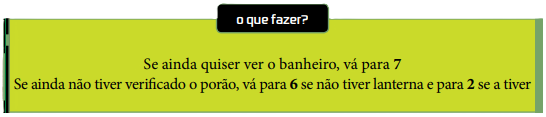
\includegraphics[scale=1]{Textuais/Pictures/Picture3.png}
	\fonte{\cite{Educacao_financeira_nas_escolas}}\label{fig:figure-3}
\end{figure}

\newpage

\section{RPG Maker MZ}
\cite(RPGMakerMZ) é uma plataforma de desenvolvimento de jogos especializada na criação de jogos de interpretação de personagens (RPG). Esta ferramenta oferece uma gama de recursos pré-construídos, tornando-a ideal para desenvolvedores que desejam criar experiências interativas sem a necessidade de uma formação técnica profunda em programação.

\subsection{Adequação para Educação Financeira}
A escolha do \cite(RPGMakerMZ) para este projeto se deve à sua capacidade de criar cenários interativos e narrativas envolventes. Essas características são cruciais para o ensino de conceitos de educação financeira para alunos do 5º ano do Ensino Fundamental. A plataforma permite a incorporação de múltiplos cenários e decisões baseadas em escolhas, que podem ser alinhadas com os princípios e objetivos da Estratégia Nacional de Educação Financeira (ENEF).

\subsection{Recursos e Funcionalidades}
O RPG Maker MZ oferece uma série de recursos que facilitam a criação de um ambiente educacional interativo. Entre eles estão:

\begin{itemize}
	\item \textbf{Eventos e Cenas:} Facilita a criação de eventos que podem desencadear diálogos, mudanças no ambiente ou outros cenários, tornando o jogo dinâmico e interativo.
	\item \textbf{Trilhas Sonoras:} Suporta a inclusão de áudio, o que pode ser usado para melhorar a imersão e o engajamento.
	\item \textbf{Personalização Visual:} Oferece uma ampla gama de opções para personalizar personagens e cenários, o que é crucial para tornar o conteúdo relatable para o público-alvo.
\end{itemize}

\subsubsection{Tilesets e Spritesheets}
\textit{Tilesets} materializam-se como conjuntos de \textit{Tiles}, onde cada \textit{Tile} representa um componente de arte \textit{pixel art} na tela, convergindo para a construção dos cenários. A possibilidade de dispor cada \textit{Tile} de maneira aleatória no \textit{Tilemap} introduz variações no leiaute do ambiente virtual. Elementos cruciais como paletas de cores do jogo e da tela são concebidos a partir da imagem central do jogador. Esta abordagem eficaz viabiliza ambientes visuais multifacetados e dinâmicos, ao passo que mantém a flexibilidade de arranjo dos elementos. Em essência, \textit{Tilesets} foram pensados como ferramentas essenciais para os criadores de jogos, permitindo a elaboração de mundos cativantes e esteticamente agradáveis por meio do encaixe estratégico de componentes \textit{pixel art} \cite{borges2021desenvolvimento}.

Complementando a funcionalidade dos \textit{Tilesets}, \textit{Spritesheets} emergem como coleções de elementos 2D que descrevem as movimentações possíveis para um personagem ou objeto no contexto do jogo. Este recurso ostenta um valor inestimável para os artistas que almejam conceber imagens dinâmicas valendo-se de ferramentas convencionais. Ao otimizar tanto os custos de produção quanto a simplicidade na geração de imagens de alta qualidade, \textit{Spritesheets} fomentam modificações na aparência e comportamento de um objeto por meio de variações de poses. A geração automática de poses intermediárias potencializa a eficiência do processo criativo. A harmonização entre \textit{Spritesheets} e \textit{Tilesets} capacita os desenvolvedores a criar experiências visuais enriquecedoras, enraizando maior interatividade e imersão no universo dos jogadores \cite{jones2013dynamic}.

\subsection{Integração com a ENEF}
A flexibilidade do RPG Maker MZ permite que o jogo seja projetado de forma a estar em conformidade com os materiais e diretrizes da ENEF. Isso garante que o jogo não seja apenas educativo, mas também metodologicamente sólido e alinhado com os padrões nacionais de educação financeira.

\begin{figure}[ht]
	\centering
	\caption{Interface do RPG Maker MZ.}
	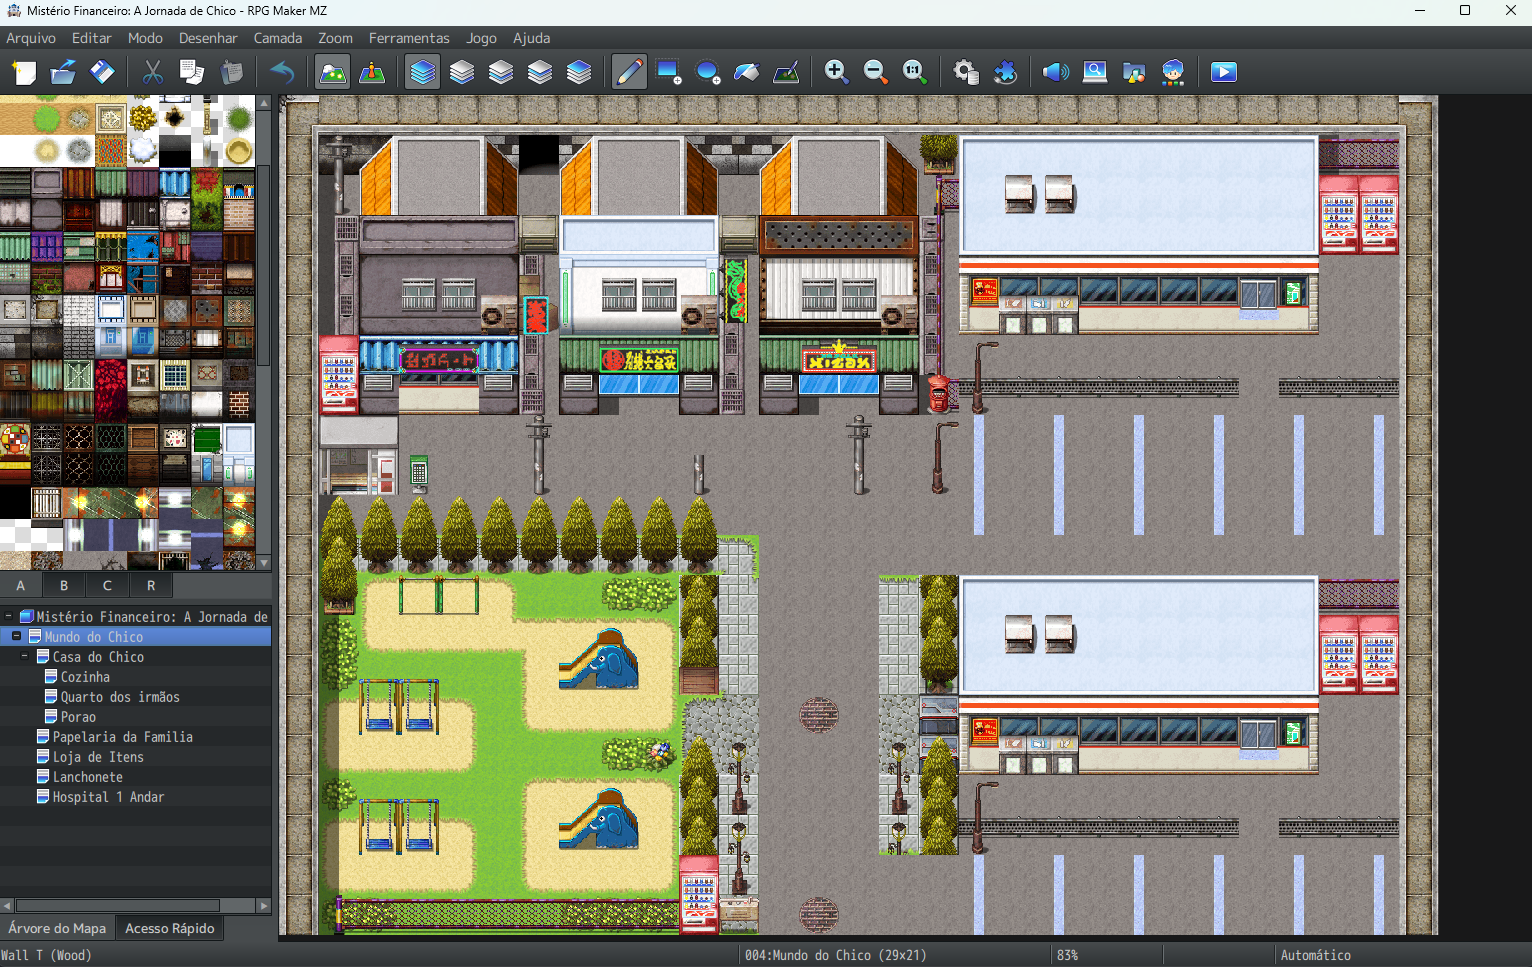
\includegraphics[scale=0.3]{Textuais/Pictures/RPGMaker_Interface.png}
	\fonte{Captura de tela do autor (2023).}\label{fig:rpgmaker-interface}
\end{figure}


\begin{figure}[ht]
	\centering
	\caption{\textit{Spritesheet.}}
	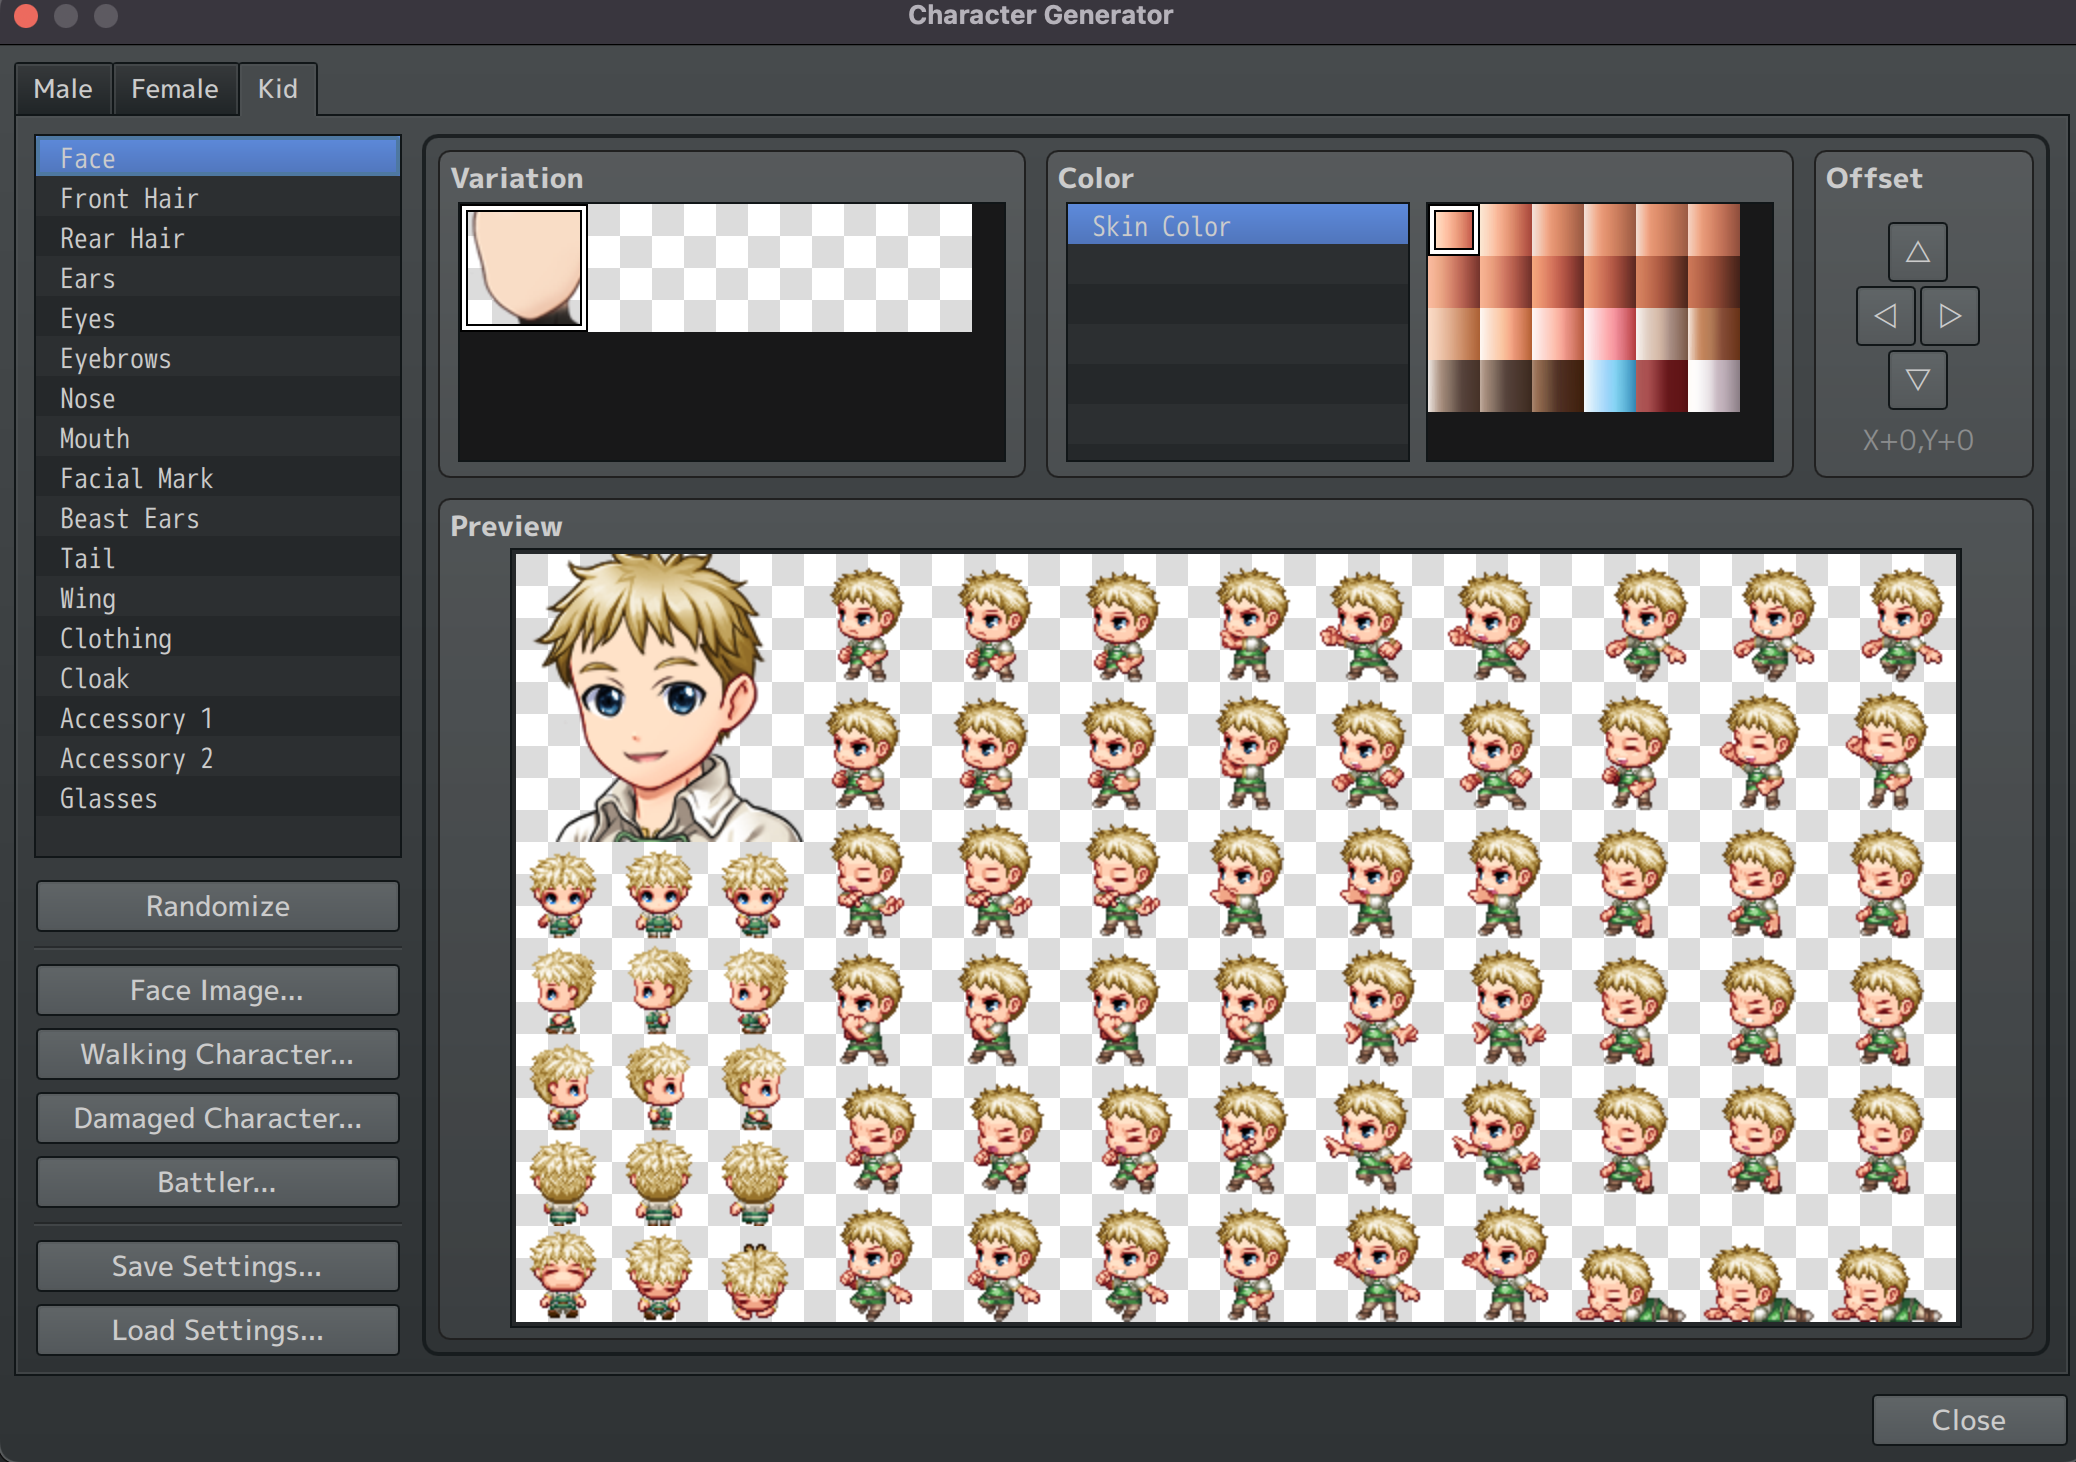
\includegraphics[scale=1.8]{Textuais/Pictures/Picture5.png}
	\fonte{\cite{RPGMakerMZ}}\label{fig:figure-5}
\end{figure}


\section{Trabalhos Correlatos}
Nesta seção serão apresentados alguns trabalhos, que de alguma maneira se correlaciona com o presente trabalho.

\subsection{Debt Maze}
O \textit{Debt Maze}\cite{Debt_Maze} é um jogo projetado para ensinar conceitos financeiros de maneira envolvente. Com um labirinto repleto de desafios baseados em temas financeiros como empréstimos, juros e pagamentos em atraso, o jogo se adapta a jogadores de todos os níveis, desde novatos até os mais familiarizados com finanças. Navegar corretamente pelo labirinto é paralelo a tomar decisões financeiras acertadas na vida real. Integrando elementos imersivos, persuasivos e personalizáveis, \textit{Debt Maze}\cite{Debt_Maze} não somente entretém, mas também visa aprimorar a alfabetização financeira do jogador, equipando-o para tomar decisões mais informadas.

Comparado ao \textit{Debt Maze}\cite{Debt_Maze}, que utiliza um labirinto para simbolizar os desafios financeiros, o presente trabalho adota uma abordagem mais prática e aplicável à vida cotidiana das crianças. Em vez de um jogo baseado em labirintos, o presente trabalho oferece cenários práticos e ferramentas para realizar escolhas financeiras reais, tornando o aprendizado mais direto.

\subsection{PlanCash}
O \textit{PlanCash}\cite{mariano2020educaccao} é um jogo de tabuleiro inovador, projetado para combinar aprendizado e diversão para o público infantil. Ele incorpora conteúdos convencionais de matemática e situações cotidianas, abordando tópicos como história do dinheiro, gestão financeira, economia e operações matemáticas básicas. Por meio de caminhos alternativos no tabuleiro, os jogadores são desafiados por cartas que propõem situações-problema, gerando reflexão e análise sobre cada proposta. As cartas, classificadas como Pergunta, Pagar, Receber, Recompensa e Roleta, oferecem uma dinâmica envolvente, onde as decisões dos jogadores influenciam seu progresso. Uma ferramenta educativa e lúdica, o \textit{PlanCash}\cite{mariano2020educaccao} é uma adição valiosa para o ensino fundamental e para famílias que buscam uma maneira divertida de ensinar conceitos financeiros e matemáticos às crianças.

O \textit{PlanCash}\cite{mariano2020educaccao} oferece uma proposta lúdica por meio de um jogo de tabuleiro, combinando educação e entretenimento para crianças. No  entanto, o presente trabalho busca evoluir esse conceito, apresentando um formato digital, que é naturalmente mais atraente para a geração atual de crianças. A digitalização não apenas moderniza a proposta, mas também incorpora elementos visuais e interativos que ampliam a experiência educacional, tornando o aprendizado sobre finanças e matemática ainda mais envolvente.

\subsection{Finance Game}
O \textit{Finance Game}\cite{Finance_Game}, desenvolvido como ferramenta educacional, aborda a gestão financeira de forma lúdica e interativa, buscando conscientizar os jogadores sobre a importância do equilíbrio entre a tomada de decisões financeiras e outros aspectos que impactam a qualidade de vida. Introduzindo os jogadores a cenários simulados da vida de um trabalhador adulto, como a administração de um orçamento pessoal e as implicações de escolhas de consumo, o jogo promove a reflexão sobre responsabilidade financeira e a busca por satisfação pessoal. Via interações com diversos elementos, como o mercado, banco e lanchonete, os jogadores são desafiados a tomar decisões que influenciam diretamente a sua situação econômica e bem-estar. O jogo visa a capacitar os jogadores a compreender as consequências de suas ações financeiras, incentivando a tomada de decisões informadas e ponderadas no mundo real.

Ao comparar o \textit{Finance Game}\cite{Finance_Game} com o presente trabalho, destaca-se que a abordagem escolhida busca proporcionar uma imersão mais profunda ao contextualizar situações financeiras na realidade da criança. Isso cria uma conexão direta com suas experiências, permitindo decisões mais identificáveis e uma compreensão prática dos princípios de educação financeira.

\subsection{InvestPlay}
O \textit{InvestPlay}\cite{santos2020investplay} é um jogo educacional que ensina educação financeira de maneira dinâmica. Os jogadores movem um personagem por casas, respondendo perguntas e tomando decisões sobre gastos e investimentos. O objetivo é equilibrar ativos e passivos, aprendendo sobre finanças. A jogabilidade é elogiada, mas o nível de algumas perguntas é desafiador para crianças. O jogo oferece personalização para diferentes temas educativos.

O \textit{InvestPlay}\cite{santos2020investplay} se destaca por sua abordagem educativa em finanças. Contudo, o presente trabalho, fundamentado na literatura da ENEF, busca refinar essa proposta. Direcionando o conteúdo especificamente para o entendimento infantil, propomos uma abordagem que simplifica conceitos, tornando-os mais acessíveis e pertinentes ao público infantil. Assim, a intenção é que as crianças assimilem os conceitos financeiros de maneira mais eficaz e contextualizada.

\subsection{Considerações sobre os Trabalhos Correlatos}

A seção de trabalhos correlatos apresenta uma variedade de abordagens utilizadas para educar e capacitar indivíduos no domínio financeiro. O exemplo do \textit{Debt Maze} ilustra a eficácia de usar mecânicas de jogos para tornar o aprendizado de conceitos financeiros mais envolvente e compreensível. Navegar por um labirinto, por exemplo, pode simbolizar os desafios financeiros e decisões que as pessoas enfrentam na vida real. A integração de elementos imersivos e persuasivos nos jogos não apenas entretém, mas também tem o potencial de aprimorar significativamente a alfabetização financeira do jogador.

Através da análise destes trabalhos, fica evidente que a gamificação é uma ferramenta poderosa para educar e capacitar as pessoas a tomar decisões financeiras mais informadas. No entanto, cada jogo ou abordagem tem suas particularidades, e a eficácia de cada um pode variar com base no público-alvo e nos objetivos de aprendizado pretendidos.

\subsection{Considerações sobre os Trabalhos Correlatos}

%Os trabalhos correlatos aqui analisados demonstram a ampla variedade de abordagens utilizadas para a educação financeira por meio de ferramentas lúdicas. A diversidade de estratégias, cenários, e sistemas de aprendizado evidencia a crescente necessidade de adaptar a instrução financeira aos diferentes públicos-alvo e contextos de vida. O jogo, como meio interativo, apresenta-se como um instrumento poderoso para tal tarefa.

%O \textit{Finance Game} destaca-se pela sua abordagem prática ao retratar cenários financeiros que se alinham diretamente com as experiências cotidianas das crianças. Ao fazer isso, ele constrói uma ponte entre teoria e prática, permitindo que os jogadores absorvam conhecimentos de forma mais eficaz. O \textit{Debt Mazer}, por sua vez, utiliza um ambiente de labirinto para representar os desafios financeiros, enfatizando a importância da tomada de decisão informada, enquanto elementos de imersão e personalização intensificam a experiência educacional.

\begin{table}[!htbp]
	\centering
	\renewcommand{\arraystretch}{1.3}
	\caption{Comparativo dos Trabalhos Correlatos com o Presente Trabalho}
	\label{tab:comparativo-trabalhos}
	\begin{tabular}{| L{2.5cm} | L{2.5cm} | L{2.5cm} | L{2.5cm} | L{2.5cm} | L{2.5cm} |}
		\hline
		\textbf{}                & \textbf{Debt Maze}       & \textbf{PlanCash}                    & \textbf{Finance Game}        & \textbf{InvestPlay}               & \textbf{Presente Trabalho}          \\
		\hline
		\hline
		\textbf{Público-Alvo}    & Geral                    & Infantil                             & Geral                        & Geral                             & Infantil                            \\
		\hline
		\textbf{Metodologia}     & Labirinto                & Jogo de Tabuleiro                    & Simulação                    & Perguntas e Respostas             & Choice-based Game                   \\
		\hline
		\textbf{Resultados}      & Alfabetização Financeira & Conhecimento Financeiro e Matemático & Tomada de Decisão Financeira & Entendimento de Ativos e Passivos & Alfabetização Financeira Interativa \\
		\hline
		\textbf{Baseado na ENEF} & Não                      & Não                                  & Não                          & Não                               & Sim                                 \\
		\hline
	\end{tabular}
	\vspace{2mm}
	\fonte{Elaborado pelo autor (2023).}
\end{table}
